\hypertarget{decode_8cpp}{}\section{decode.\+cpp File Reference}
\label{decode_8cpp}\index{decode.\+cpp@{decode.\+cpp}}
{\ttfamily \#include \char`\"{}decode.\+h\char`\"{}}\\*
{\ttfamily \#include $<$stdio.\+h$>$}\\*
Include dependency graph for decode.\+cpp\+:\nopagebreak
\begin{figure}[H]
\begin{center}
\leavevmode
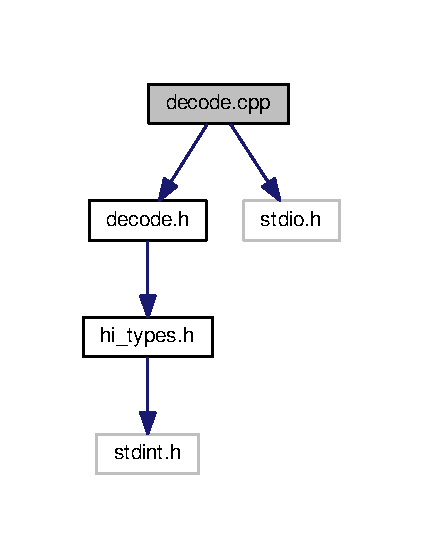
\includegraphics[width=203pt]{decode_8cpp__incl}
\end{center}
\end{figure}


\subsection{Detailed Description}
Process raw files from the \hyperlink{classFC5025}{F\+C5025}, and decode either F\+M or M\+F\+M encoded buffers. 